%
% File acl2019.tex
%
%% Based on the style files for ACL 2018, NAACL 2018/19, which were
%% Based on the style files for ACL-2015, with some improvements
%%  taken from the NAACL-2016 style
%% Based on the style files for ACL-2014, which were, in turn,
%% based on ACL-2013, ACL-2012, ACL-2011, ACL-2010, ACL-IJCNLP-2009,
%% EACL-2009, IJCNLP-2008...
%% Based on the style files for EACL 2006 by 
%%e.agirre@ehu.es or Sergi.Balari@uab.es
%% and that of ACL 08 by Joakim Nivre and Noah Smith

\documentclass[11pt]{article}
%%\usepackage[hyperref]{acl2019}
\usepackage{times}
\usepackage{amsmath}
\usepackage{amssymb}
\usepackage{latexsym}
\usepackage{lingstyle}
\usepackage{graphicx}
\usepackage{tikz}
\usepackage{bussproofs}
\usepackage[margin=0.5in]{geometry}
\usetikzlibrary{arrows,positioning,shapes} 
\tikzset{
    %Define standard arrow tip
    >=stealth',
    %Define style for boxes
    amrnode/.style={
             ellipse,
             draw=black, very thick,
             font=\small},
    scopenode/.style={
             ellipse,
             draw=red, very thick, dashed,
             text=red,
             font=\small},
    % Define arrow style
    amrarrow/.style={
            ->,
            thick,
            font=\small},
    scopearrow/.style={
              ->,
              red,
              thick,
              dashed,
              font=\small}
}



 \def\drs#1#2{\begin{tabular}{|l|}\hline #1 \\ \hline \\
                [-8pt] #2\\[-8pt] \\ \hline \end{tabular} }

 \def\ddrs#1{\begin{tabular}{||c||}\hline \\
                [-8pt] #1\\[-8pt] \\ \hline \end{tabular} }

 \def\topdrs#1#2{\begin{tabular}{|l|}\hline #1 \\ \hline \\
                [-8pt] #2 \\[-8pt] \\ \hline \end{tabular} }

 \def\proof#1#2#3#4{\drs{#1}{#2} \ $\vdash$ \ \drs{#3}{#4}}
 \def\modimp#1#2#3#4{\mbox{\drs{#1}{#2} \ $\Box$ \ \drs{#3}{#4}}}
 \def\imp#1#2#3#4{\drs{#1}{#2} \ $\Rightarrow$ \ \drs{#3}{#4}}
 \def\dis#1#2#3#4{\mbox{\drs{#1}{#2} \ $\vee$ \ \drs{#3}{#4}}}
 \def\int#1#2{\mbox{$^{\wedge}$ \ \drs{#1}{#2}}}
 \def\pos#1#2{\mbox{$\Diamond$ \ \drs{#1}{#2}}}
 \def\nec#1#2{\mbox{$\Box$ \ \drs{#1}{#2}}}
 \def\nega#1#2{\mbox{$\neg$ \ \drs{#1}{#2}}}
 \def\pred#1#2#3{\mbox{#1\ :\drs{#2}{#3}}}


\usepackage{url} 

\usepackage[acronym]{glossaries} % 'nomain' to disable automatic generation of "glossary" section 
\glsdisablehyper % disable hyperlink to non-existing glossary section 
%\aclfinalcopy % Uncomment this line for the final submission
%\def\aclpaperid{***} %  Enter the acl Paper ID here

%\setlength\titlebox{5cm}
% You can expand the titlebox if you need extra space
% to show all the authors. Please do not make the titlebox
% smaller than 5cm (the original size); we will check this
% in the camera-ready version and ask you to change it back.

\newcommand\BibTeX{B\textsc{ib}\TeX}

\title{Modeling Quantification and Scope in Abstract Meaning Representations
%Towards a Unified Meaning Representation for Quantification
}
 

 
\author{
  Eli Goldner
}
\begin{document}
\maketitle



\enumsentence{
Carl submitted the forms and everyone will sign up again tomorrow.
\label{submit-1}}

\enumsentence{
  
  a.
  \scriptsize\texttt{(a / and\\
    \hspace*{0.5cm}:op1 (f / fill-out-03 :ongoing - :complete + :time (b / before :op1 (n / now))\\
    \hspace*{1.0cm}:ARG0 (p1 / person\\
    \hspace*{1.5cm}:name (n / name\\
    \hspace*{2.0cm}:op "Carl"))\\
    \hspace*{1.0cm}:ARG1 (f / form))\\
    \hspace*{0.5cm}:op2 (s / scope\\
    \hspace*{1.0cm}:pred (m / submit-01  :ongoing - :complete + :time (a / after :op1 (n / now))\\
    \hspace*{1.5cm}:ARG0 (p / person\\
    \hspace*{2.0cm}:mod (a / all))\\
    \hspace*{1.5cm}:ARG1 f)))\\}
  





\enumsentence{
John can't afford a car at the moment.
\label{afford-1}}

\enumsentence{
  
  a.
  \small\texttt{(p / possible-01\\
    \hspace*{1.0cm}:ARG0 (a / afford-01\\
    \hspace*{1.5cm}:ARG0 (p2 / person\\
    \hspace*{2.0cm}:name (n / name\\
    \hspace*{2.5cm}:op "John"))\\
    \hspace*{1.5cm}:ARG1 (c /car)\\
    \hspace*{1.5cm}:time (m / moment))\\
    \hspace*{1.0cm}:polarity -)}
  
  b.
  \\
  
  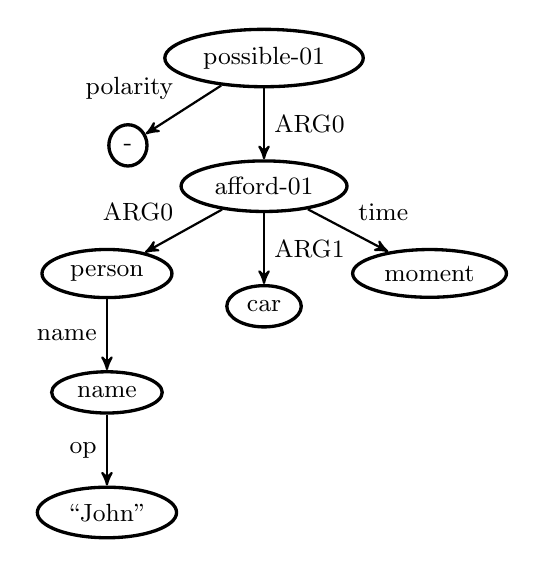
\begin{tikzpicture}[node distance=0.9cm, auto,]
    \node[amrnode] (possible) {possible-01};
    \node[amrnode, below left=0.9cm of possible] (neg) {-};
    \node[amrnode, below=0.9cm of possible] (afford) {afford-01};
    \node[amrnode, below left=0.9cm of afford] (person) {person};
    \node[amrnode, below =0.9cm of afford] (car) {car};
    \node[amrnode, below right=0.9cm of afford] (moment) {moment};
    \node[amrnode, below =0.9cm of person] (name) {name};
    \node[amrnode, below =0.9cm of name] (john) {``John''};
    \path (possible) edge[amrarrow] node[auto] {ARG0} (afford)
    (possible) edge[amrarrow] node[above left] {polarity} (neg)
    (afford) edge[amrarrow] node[above left] {ARG0} (person)
    (afford) edge[amrarrow] node[auto] {ARG1} (car)
    (afford) edge[amrarrow] node[auto] {time} (moment)
    (person) edge[amrarrow] node[left] {name} (name)
    (name) edge[amrarrow] node[left] {op} (john);
  \end{tikzpicture}
  \label{afford-AMR}}

\enumsentence{
%\setlength\itemsep{-5pt}
\item {\bf afford-01}: be able to spare, have the financial means
\\ {\tt\small ARG0:} haver of financial means, agent \\
  {\tt\small ARG2:} costly thing, theme

\item {\bf afford-02}: provide, make available
\\
 {\tt\small ARG0:} provider, agent
\\
{\tt\small ARG1:} provided, theme
\\
{\tt\small ARG2:} recipient
 
}


The attraction of AMR-style representations and annotations is the adoption of a {\it predicative core} element along with its arguments: e.g., an event and its participants. This, in turn, leads to an event-rooted graph that has many advantages for parsing and matching algorithms. As can be seen from the example, the predicate-argument structure is front and center in AMR, and we consider this to be one of its strengths.

However, as it currently stands, AMR does not represent quantification or its interaction with modality and negation \cite{bos2016expressive}. The challenge is to maintain the focus on the predicate-argument structure while also adequately accounting for linguistic phenomena that operate above the level of the core AMR representation, in particular quantification and modality.

\section{Quantification and Scope}

 
 It can be argued that, besides graph-based matching over predicative structures, AMR does not provide good support for logical inference because it does not yet properly handle scoping and other phenomena. For example, in (\ref{talk}), there is a single talk that everyone in the room is listening to, while in (\ref{coffee}), each person has their own coffee. However, AMR does not distinguish between these two cases: it could just as well be that everyone in the room listened to a different talk, or that everyone at noon shared a single cup of coffee.
 
\enumsentence{
a. Everyone in the room  listened  to a talk. 
\\
b. $\exists y[\mbox{talk}(y)\hspace*{-1mm} \wedge \forall x\exists e[\mbox{person}(x)\hspace*{-1mm} \wedge \hspace*{-1mm}\mbox{inRoom}(x) \rightarrow \mbox{listen}(e,x,y)] ]$
\\
c. \small\texttt{(l / listen-01\\
\hspace*{1.0cm}:ARG0 (p / person\\
\hspace*{1.5cm}:mod (a / all)\\
\hspace*{1.5cm}:location (r / room))\\
\hspace*{1.0cm}:ARG1 (t / talk))
}
\label{talk}}

\enumsentence{
a. Everyone drank a coffee at noon. 
\\
b. $\forall x[\mbox{person}(x) \rightarrow \exists y\exists e[\mbox{coffee}(y) \wedge \mbox{drink}(e,x,y)\wedge @(e,\mbox{noon})]] $
\\
c. \small\texttt{(d / drink-01\\
\hspace*{1.0cm}:ARG0 (p / person\\
\hspace*{1.5cm}:mod (a / all))\\
\hspace*{1.0cm}:ARG1 (c / coffee)\\
\hspace*{1.0cm}:time (n / noon))
}
\label{coffee}}

\noindent

 
In fact, this inability of AMRs to distinguish scoping relations among quantifiers also extends to negation and modality. For example, the AMR for the sentence ``Every student did not fail" is given below.

\enumsentence{
a. \small\texttt{(d / fail-01\\
\hspace*{0.5cm}:ARG0 (s / student\\
\hspace*{1.0cm}:mod (a / all))\\
\hspace*{0.5cm}:polarity -)
}\\
{\normalsize b.} \\ 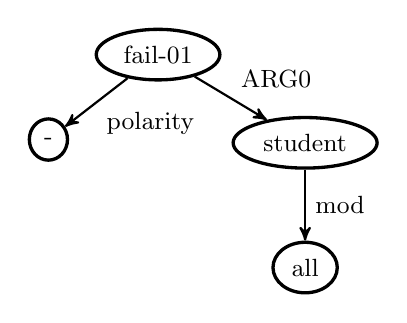
\begin{tikzpicture}[node distance=0.9cm, auto,]
 %\node[scopenode] (scope) {scope};
 \node[amrnode] (fail) {fail-01};
 \node[amrnode, below left=0.9cm of fail] (neg) {-};
 \node[amrnode, below right=0.9cm of fail] (student) {student};
 \node[amrnode, below=0.9cm of student] (all) {all};
 \path %(scope) edge[scopearrow] node[auto] {pred} (fail)
       %(scope) edge[scopearrow, bend right=45] node[left] {ARG0} (neg)
       %(scope) edge[scopearrow, bend left=45] node[auto] {ARG1} (student)
       (fail) edge[amrarrow] node[auto] {polarity} (neg)
       (fail) edge[amrarrow] node[auto] {ARG0} (student)
       (student) edge[amrarrow] node[auto] {mod} (all);
\end{tikzpicture}
\label{picture3}}

\noindent
The sentence is ambiguous, however, between the readings ``for every student, that student did not fail" and ``it is not the case that every student failed".

While MRS and other flattened semantic representations provide a solution to these issues, giving faithful translations of scope with typed expressions, there are several drawbacks to these approaches.  Flat representations reveal no semantic core. Hence, as annotations, the resulting structures are difficult to interpret and inspect.  Furthermore, quantifier scope is often underspecified even when it can be disambiguated in context. 
Dependency MRS (DMRS) is one  exception to this in the MRS family of representations \cite{copestake2009slacker}, where dependency relations link argument heads to the major predicator of the sentence.

In our research, we propose to represent scope relationally, while maintaining both the centrality of the predicative core of the sentence (e.g., {\it listen}, {\it drink}), as well as the syntactic integrity of the quantified expression  (e.g., {\it every person}). A relational interpretation for scope provides a first-order interpretation: it references two specific nodes in the graph, and orders one relative to the other. This operates over generalized quantifiers ({\it some book}, {\it most people}), negation ({\it not}, {\it no}), as well as modals ({\it possibly}, {\it likely}, {\it must}). From an annotation perspective, this is quite different from flat structures, since a human judgment in scope between two elements is directly reflected in the resulting graph. There are complex interactions between negation, modal expressions, and quantified NPs that we will examine, first representationally, and then experimentally with small-scale annotation and testing. 



\iffalse
Quantifier Scope examples: the data are suggestive that non-deafult scopes are not uncommon, and depend on context and predicative preferences. 





\eenumsentence{

\item In privatized societies, everybody tramples over someone trying to maximize their own interests.
\item An earthquake in Sichuan stunned everyone.
\item The real estate phenomenon exists in every sector of the national economy.
\item Every year, all levels of People's Congress are held in the country.
}


Negation Lowering and Implicature

\eenumsentence{

\item We don't want to revitalize the nation through trials and tribulations \\
{\bf presup}: $want(we,\;^{\hat{}}\exists x,e[revitalize(e,we,Nation) \wedge means(e,x)])$ \\
$\mathring{{\bf but}}$  $\neg [trial(x) \vee tribulation(x)]$
\item He doesn't want to have dinner at the Thai restaurant. \\
{\bf presup}: $want(he,\;^{\hat{}}\exists x,e[dine(e,he) \wedge locate(e,x)])$ \\
$\mathring{{\bf but}}$  $\neg [Thai\_Restaurant(x)]$
\item I don't want you going to university in Europe. \\
{\it ditto}
}




Neg-Raising \`{a} la Horn

\eenumsentence{

\item Bill doesn't think that Mary likes fish. \\
{\bf presup}: $think(Bill, \;^{\hat{}}\neg (like(Mary,fish))$
\item Bill doesn't think Mary will leave until tomorrow. 
\item {\bf but not}: Bill didn't say Mary was here.

%\end{itemize}
}



Events and quantification

\eenumsentence{

\item John left Boston for New York. \\
{\bf presup} $\exists x[loc(x,John) \wedge x \neq Boston]$ \\
$\exists x, e_1,e_2[at(e_1,John,Boston) \wedge at(e_2,John,x) \wedge e_1 < e_2]$
\item Mary arrived in New York from Boston.
\item A crowd assembled on the Mall.
\item The students ate lunch in the mensa.
\item Bill painted a portrait. 
\item The door closed. 
\item John walked for hours in the park.
}
\fi

 
We believe there are advantages to adopting an AMR-style representation for predicate-argument forms of sentences \cite{banarescu2013abstract}. Given the complexity inherent in the semantics of number, negation, and quantification, we  believe that a similar approach to the annotation of scope has some advantages. These include the following:

\begin{itemize}

\item It maintains a focus on the  {\it predicative core} of the sentence;
\item There is likely a lower {\it cognitive load} for annotation by non-experts;
\item Semantic relations are {\it transparent} in the graphical representation.
\end{itemize}

\noindent Addressing the problems associated with scope adopting this approach results in a   representation  we call ``Uniform Meaning Representation" (UMR), where the predicative core of AMR is maintained, and embedded  under a ``scope" graph when required.



\section{Towards a Uniform Meaning Representation for Scope}
\label{sec:umr}
 
 In this section, we illustrate our approach to encoding the expression of quantifier scope in UMR. We draw on some work within the ISO annotation community, where the problem of explicitly annotating scoping relations of events and temporal or spatial quantifiers   has been addressed.
 

 To explicitly represent relative scope of quantified expressions, 
ISO-Space \cite{pustejovsky2017iso} uses the @quant attribute (adopted from ISO-TimeML), applying it to spatial entities, and in addition uses the attribute @scopes to specify a scoping relation. The following example, taken from ISO 24617-7:2014, illustrates this:

\eenumsentence{\label{isospace}
\item A computer$_{se1}$ is on$_{ss1}$ every desk$_{se2}$. 
\vspace*{-4mm}
\item 
{\small 
     $<$spatialEntity id=``se1"   pred=``computer"\\ quant=``1'' 
       scopes=``$\emptyset$"/$>$\\
     $<$spatialEntity id=``se2" 
      \hspace*{2mm} pred=``desk" \\ quant=``every"
   scopes=``\#se1"/$>$
      %\\
    % $<$spatialSignal id=``ss1" target=``\#token3"\\
     % \hspace*{2mm} type=``dirTop" /$>$\\
     %$<$qsLink id=``qsl1" relType=``EC" figure=``\#se1"\\
     %%$<$oLink id=``ol1" relType=``above" figure=``\#se1"\\
    % \hspace*{2mm}  ground=``\#se2" trigger=``\#ss1" frameType=``intrinsic"\\
    % \hspace*{2mm} referencePt=``\#se2" projective=``false" /$>$
}}
 
 

\enumsentence{ 
a. \small\texttt{(s / scope\\
\hspace*{1.0cm}:pred (b / be-located-at-91\\
\hspace*{1.5cm}:ARG0 (c / computer)\\
\hspace*{1.5cm}:ARG1 (d / desk\\
\hspace*{2.0cm}:quant (e / every)))\\
\hspace*{1.0cm}:ARG0 d\\
\hspace*{1.0cm}:ARG1 c)}
\\\\
{\normalsize b.} \\
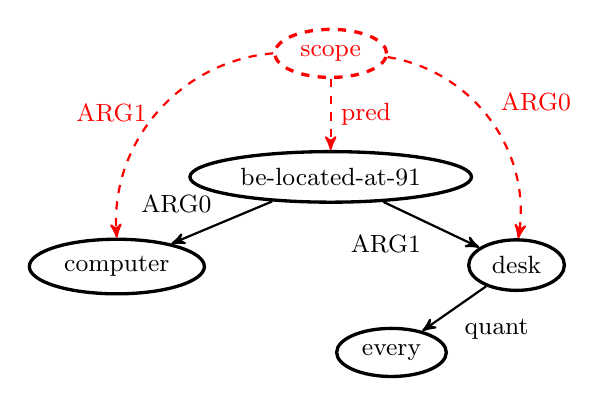
\begin{tikzpicture}[node distance=0.9cm, auto,]
 \node[scopenode] (scope) {scope};
 \node[amrnode, below=0.9cm of scope] (on) {be-located-at-91};
 \node[amrnode, below left=0.9cm of on] (computer) {computer};
 \node[amrnode, below right=0.9cm of on] (desk) {desk};
 \node[amrnode, below left=0.9cm of desk] (all) {every};
% \node[amrnode, below right=0.9cm of person] (room) {room};
 \path (scope) edge[scopearrow] node[auto] {pred} (on)
       (scope) edge[scopearrow, bend right=45] node[left] {ARG1} (computer)
       (scope) edge[scopearrow, bend left=45] node[auto] {ARG0} (desk)
       (on) edge[amrarrow] node[above left] {ARG0} (computer)
       (on) edge[amrarrow] node[below left] {ARG1} (desk)
       (desk) edge[amrarrow] node[auto] {quant} (all);
\end{tikzpicture}
\label{everycomputer}
}



\enumsentence{
a. John golfed every Sunday. \\
b. 
$\forall t[\mbox{Sunday}(t) \rightarrow \exists e[\mbox{golf}(e,j) \wedge \mbox{on}(e,t)]]$
\label{golf}
}

\enumsentence{ 
a. \small\texttt{(s / scope\\
\hspace*{1.0cm}:pred (p / possible-01\\
\hspace*{1.5cm}:ARG0 (a / afford-01\\
\hspace*{2.0cm}:ARG0 (p2 / person\\
\hspace*{2.5cm}:name (n / name\\
\hspace*{3.0cm}:op "John"))\\
\hspace*{2.0cm}:ARG1 (c /car)\\
\hspace*{2.0cm}:time (m / moment))\\
\hspace*{1.5cm}:polarity (n2 / not))\\
\hspace*{1.0cm}:ARG0 n2\\
\hspace*{1.0cm}:ARG1 p)}\\
%\newpage
{\normalsize b.} \\
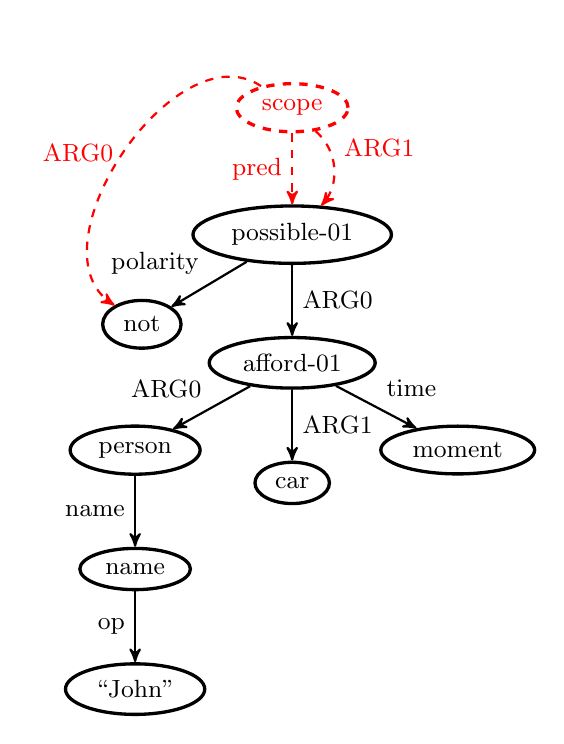
\begin{tikzpicture}[node distance=0.9cm, auto,]
 \node[scopenode] (scope) {scope};
 \node[amrnode, below=0.9cm of scope] (possible) {possible-01};
 \node[amrnode, below left=0.9cm of possible] (neg) {not};
 \node[amrnode, below=0.9cm of possible] (afford) {afford-01};
 \node[amrnode, below left=0.9cm of afford] (person) {person};
 \node[amrnode, below =0.9cm of afford] (car) {car};
 \node[amrnode, below right=0.9cm of afford] (moment) {moment};
 \node[amrnode, below =0.9cm of person] (name) {name};
 \node[amrnode, below =0.9cm of name] (john) {``John''};
 \path (scope) edge[scopearrow] node[left] {pred} (possible)
       (scope) edge[scopearrow, bend right=90] node[left] {ARG0} (neg)
       (scope) edge[scopearrow, bend left=45] node[auto] {ARG1} (possible)
       (possible) edge[amrarrow] node[auto] {ARG0} (afford)
       (possible) edge[amrarrow] node[above left] {polarity} (neg)
       (afford) edge[amrarrow] node[above left] {ARG0} (person)
       (afford) edge[amrarrow] node[auto] {ARG1} (car)
       (afford) edge[amrarrow] node[auto] {time} (moment)
       (person) edge[amrarrow] node[left] {name} (name)
       (name) edge[amrarrow] node[left] {op} (john);
\end{tikzpicture}
}

\enumsentence{
$\neg  \Diamond [\exists x[\mbox{car}(x) \wedge  \exists e[\mbox{afford}(e,j,x) \hspace*{-1mm}
\wedge @(e,\mbox{N})]]$

}

\enumsentence{

$\neg  \exists x[\mbox{car}(x) \wedge \Diamond \exists e[\mbox{afford}(e,j,x) \hspace*{-1mm}
\wedge @(e,\mbox{N})]]$
\label{QML1}}


\enumsentence{ $\;$ \\
\begin{tikzpicture}[node distance=0.9cm, auto,]
 %\node[scopenode] (scope) {scope};
 \node[amrnode, below=0.9cm of scope] (survive) {survive-01};
 \node[amrnode, below left=0.9cm of survive] (neg) {-};
 \node[amrnode, below right=0.9cm of survive] (passenger) {passenger};
 \path %(scope) edge[scopearrow] node[auto] {pred} (survive)
       %(scope) edge[scopearrow, bend right=45] node[left] {ARG0} (neg)
       %(scope) edge[scopearrow, bend left=45] node[auto] {ARG1} (passenger)
       (survive) edge[amrarrow] node[auto] {polarity} (neg)
       (survive) edge[amrarrow] node[auto] {ARG0} (passenger);
\end{tikzpicture}
\label{survive}
}

 
\enumsentence{ $\;$ \\
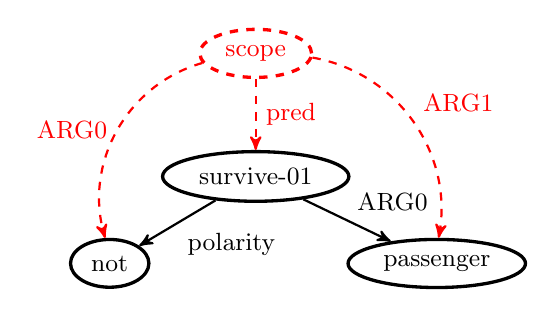
\begin{tikzpicture}[node distance=0.9cm, auto,]
 \node[scopenode] (scope) {scope};
 \node[amrnode, below=0.9cm of scope] (survive) {survive-01};
 \node[amrnode, below left=0.9cm of survive] (neg) {not};
 \node[amrnode, below right=0.9cm of survive] (passenger) {passenger};
 \path (scope) edge[scopearrow] node[auto] {pred} (survive)
       (scope) edge[scopearrow, bend right=45] node[left] {ARG0} (neg)
       (scope) edge[scopearrow, bend left=45] node[auto] {ARG1} (passenger)
       (survive) edge[amrarrow] node[auto] {polarity} (neg)
       (survive) edge[amrarrow] node[auto] {ARG0} (passenger);
\end{tikzpicture}
}


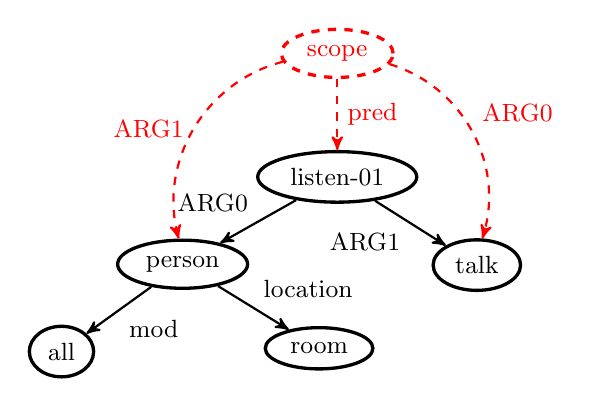
\begin{tikzpicture}[node distance=0.9cm, auto,]
 \node[scopenode] (scope) {scope};
 \node[amrnode, below=0.9cm of scope] (listen) {listen-01};
 \node[amrnode, below left=0.9cm of listen] (person) {person};
 \node[amrnode, below left=0.9cm of person] (all) {all};
 \node[amrnode, below right=0.9cm of person] (room) {room};
 \node[amrnode, below right=0.9cm of listen] (talk) {talk};
 \path (scope) edge[scopearrow] node[auto] {pred} (listen)
       (scope) edge[scopearrow, bend right=45] node[left] {ARG1} (person)
       (scope) edge[scopearrow, bend left=45] node[auto] {ARG0} (talk)
       (listen) edge[amrarrow] node[above left] {ARG0} (person)
       (listen) edge[amrarrow] node[below left] {ARG1} (talk)
       (person) edge[amrarrow] node[auto] {mod} (all)
       (person) edge[amrarrow] node[auto] {location} (room);
\end{tikzpicture} 

\end{document}
